\documentclass[mathNotesPreamble]{subfiles}
\begin{document}
%\relscale{1.4}
\section{4.2: Mean Value Theorem}
Before studying the \textit{Mean Value Theorem}, we must first learn \textit{Rolle's Theorem}:\\

\begin{thmBox*}[Theorem 4.3: Rolle's Theorem]
  Let $f$ be continuous on a closed interval $[a,b]$ and differentiable on $(a,b)$ with $f(a)=f(b)$. There is at least one point $c$ in $(a,b)$ such that $f'(c)=0$.
\end{thmBox*}

\begin{center}
  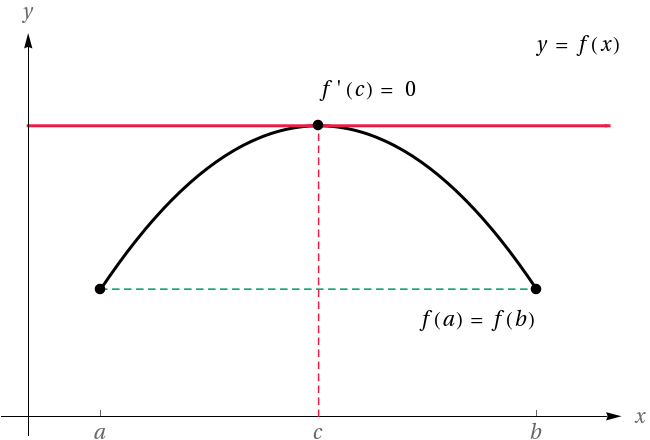
\includegraphics[width=0.3\linewidth]{images/briggs_04_02/RollesThm01.png}
\end{center}

\textit{Note:} Rolle's Theorem requires $f$ be both \textit{continuous} and \textit{differentiable}:
\begin{center}
  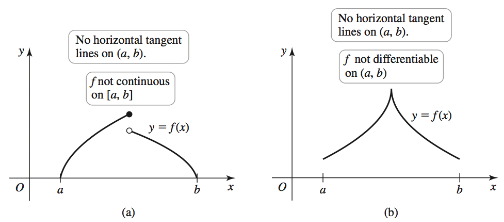
\includegraphics[width=0.6\linewidth]{images/briggs_04_02/RollesThm02.png}
\end{center}

\begin{ex*}
  Determine whether Rolle's Theorem applies for the following. If it applies, find the point(s) $c$ such that $f'(c)=0$.
\end{ex*}
$f(x)=\sin(2x)$ on $\sbrkt{0, \frac{\pi}{2}}$
\pagebreak

\begin{thmBox*}[Theorem 4.4: Mean Value Theorem]
  If $f$ is continuous on a closed interval $[a,b]$ and differentiable on $(a,b)$, then there is at least one point $c$ in $(a,b)$ such that 
$\frac{f(b)-f(a)}{b-a}=f'(c)$.
\end{thmBox*}

\begin{center}
  \begin{tikzpicture}
    \begin{axis}[declare function={
      f(\x)=(\x)*(\x-1.5)*(\x-2);
      fp(\x)=3*(\x)^2-7*(\x)+3;
      a=0.125; b=0.875; c=0.4657248399474699;},
      axis lines=center,
      axis line style={->},
      width=0.4\linewidth,
      xmin=-0.25, xmax=2.25,
      ymin=-0.5, ymax=1.2,
      ticklabel style={font=\footnotesize,inner sep=0.5pt,fill=white,opacity=1.0, text opacity=1},
      xlabel=$x$, xlabel style={at={(ticklabel* cs:1)},anchor=north west},
      ylabel=$y$, ylabel style={at={(ticklabel* cs:1)},anchor=south west},
      every axis plot/.append style={line width=0.95pt, color=blue, samples=100}
      ]
      \addplot[-] expression[domain=-0.2:2.5]{f(x)};
      \addplot[-, red] expression[domain=-0.2:2.5]{fp(c)*(x-c)+f(c)};                %tangent line
      \addplot[densely dashed, black] expression[domain=-0.2:2.5]{fp(c)*(x-a)+f(a)}; %secant line
      \addplot[soldot, black] coordinates{(a,{f(a)})} node[below right, xshift=-2pt, yshift=4pt] {$A$};
      \addplot[soldot, black] coordinates{(b,{f(b)})} node[right, xshift=5pt, yshift=-2pt] {$B$};
      \addplot[soldot, black] coordinates{(c,{f(c)})} node[above] {$C$};
    \end{axis}
  \end{tikzpicture}
\end{center}

\begin{ex*}
  For $f(x)=x^\frac{2}{3}$ on the interval $\sbrkt{0,1}$, does the Mean Value Theorem apply? If so, find the point(s) $c$ such that $\frac{f(b)-f(a)}{b-a}=f'(c)$
\end{ex*}
\pagebreak

\begin{ex*}
  For each function, associated interval and graph determine if the conditions for the Mean Value Theorem are met and find the value(s) of $c$ such that $\dfrac{f(b)-f(a)}{b-a}=f'(c)$.
\end{ex*}
\begin{enumerate}
  \def\width{0.38\linewidth}
  \item 
    $f(x)=\dfrac{x^2}{4}+1$ on $\sbrkt{-2,4}$
    
    \begin{tikzpicture}
      \begin{axis}[
        grid=both,
        grid style={line width=0.35pt, draw=gray!75},
        axis lines=center,
        axis line style={-},
        width=\width,
        xmin=-3, xmax=5,
        ymin=0, ymax=6,
        xtick={-6,-5,...,6},
        ytick={-6,-5,...,6},
        ticklabel style={font=\footnotesize,inner sep=0.5pt,fill=white,opacity=1.0, text opacity=1},
        every axis plot/.append style={line width=0.95pt, color=blue, samples=100}
        ]
        \addplot[-] expression[domain=-3:5]{x^2/4+1};
        \addplot[-] expression[domain=-3:5, red]{0.5*x+3};
      \end{axis}
    \end{tikzpicture}
  \item 
    $f(x)=2\sqrt{x}$ on $\sbrkt{0,4}$
    
    \begin{tikzpicture}
      \begin{axis}[
        grid=both,
        grid style={line width=0.35pt, draw=gray!75},
        axis lines=center,
        axis line style={-},
        width=\width,
        xmin=0, xmax=4,
        ymin=0, ymax=4,
        xtick={-6,-5,...,6},
        ytick={-6,-5,...,6},
        ticklabel style={font=\footnotesize,inner sep=0.5pt,fill=white,opacity=1.0, text opacity=1},
        every axis plot/.append style={line width=0.95pt, color=blue, samples=501}
        ]
        \addplot[-] expression[domain=0:4]{2*sqrt(x)};
        \addplot[-] expression[domain=0:4, red]{x};
      \end{axis}
    \end{tikzpicture}
  \item 
    $f(x)=\dfrac{x^5}{16}$ on $\sbrkt{-2,2}$
    
    \begin{tikzpicture}
      \begin{axis}[
        grid=both,
        grid style={line width=0.35pt, draw=gray!75},
        axis lines=center,
        axis line style={-},
        width=\width,
        xmin=-3.5, xmax=3.5,
        ymin=-3.5, ymax=3.5,
        xtick={-6,-5,...,6},
        ytick={-6,-5,...,6},
        ticklabel style={font=\footnotesize,inner sep=0.5pt,fill=white,opacity=1.0, text opacity=1},
        every axis plot/.append style={line width=0.95pt, color=blue, samples=100}
        ]
        \addplot[-] expression[domain=-3:3]{x^5/16};
        \addplot[-] expression[domain=-3:3, red]{x};
      \end{axis}
    \end{tikzpicture}
\end{enumerate}
\pagebreak

\begin{ex*}
  Determine whether Rolle's Theorem applies to the following functions and find the point(s) $c$ if applicable.
\end{ex*}
\begin{enumerate}[itemsep=\stretch{1}]
  \item $f(x)=x(x-1)^2$ on $\sbrkt{0,1}$.
  \item $f(x)=x^3-x^2-5x-3$ on $\sbrkt{-1,3}$.
\end{enumerate}
\vspace*{\stretch{1}}

\begin{ex*}
  Determine whether the Mean Value Theorem applies to the following functions and find the point(s) $c$ if applicable.
\end{ex*}
\begin{enumerate}[itemsep=\stretch{1}]
  \item $f(x)=3x^2+2x+5$ on $\sbrkt{-1,1}$.
  \item $f(x)=x\inv[\frac{1}{3}]$ on $\sbrkt{\frac{1}{8},8}$.
\end{enumerate}
\vspace*{\stretch{1}}
\pagebreak
\begin{enumerate}[itemsep=\stretch{1}]
  \setcounter{enumi}{2}
  \item $f(x)=\begin{cases}
      \frac{\sin(x)}{x},& -\pi\leq x<0\\
      0,& x=0
    \end{cases}$.
  \item $f(x)=\abs{x-1}$ on $\sbrkt{-1,4}$.
\end{enumerate}
\vspace*{\stretch{1}}
\begin{ex*}[Mean Value Theorem and graphs]
  
  \noindent
  Locate all points on the graph at which the slope of the tangent line equals the secant line on the interval $\sbrkt{-4,4}$.
\end{ex*}
  
\begin{center}
  \begin{tikzpicture}
    \begin{axis}[
      axis lines=center,
      axis line style={->},
      xmin=-5.5, xmax=5.5,
      ymin=-3.5, ymax=4.5,
      xtick={-6,-4,...,6},
      ytick={-6,-4,...,6},
      minor x tick num=1,
      minor y tick num=1,
      ticklabel style={font=\footnotesize,inner sep=0.5pt,fill=white,opacity=1.0, text opacity=1},
      xlabel=$x$, xlabel style={at={(ticklabel* cs:1)},anchor=north west},
      ylabel=$y$, ylabel style={at={(ticklabel* cs:1)},anchor=south west},
      every axis plot/.append style={line width=0.95pt, color=blue, samples=100}
      ]
      \addplot[-] expression[domain=-4:4]{(x+3.75)*(x+1)*x*(x-3.5)/20};
      \addplot[soldot,red] coordinates{(-4,1.125)(4,3.875)};
      \draw[-] (-4,1.125)--(4,3.875);
    \end{axis}
  \end{tikzpicture}
\end{center}
\pagebreak

\begin{ex*}
  Find the number that satisfies the hypotheses of the Mean Value Theorem for $f(x)=\sqrt x$ on $\sbrkt{0,4}$. Graph the function, the secant line through the endpoints, and the tangent line at $c$, visually verify that the secant and tangent are parallel.
\end{ex*}
\vspace*{\stretch{1}}

\begin{ex*}[Drag racer acceleration]
  
  \noindent
  The fastest drag racers can reach a speed of $330\,mph$ over a quarter-mile strip in $5\,s$ (from a standing start). At some point during the race, the maximum acceleration of the drag racer is at least \underline{\hspace*{50pt}}$\,mph/s$.
\end{ex*}
\vspace*{\stretch{1}}

\begin{ex*}
  A state patrol officer saw a car start from rest at a highway on-ramp. She radioed ahead to another officer 35 miles from the on-ramp. When the car reached the location of the second officer, 30 minutes later, it was clocked going $60\,mph$. The driver of the car was given a ticket for exceeding the $65\,mph$ speed limit. Why can the officer conclude that the driver exceeded the speed limit?
\end{ex*}
\vspace*{\stretch{1}}
\pagebreak

%TODO remove relsize
\end{document}
